% --------------------------------------------------------------
% This is all preamble stuff that you don't have to worry about.
% Head down to where it says "Start here"
% --------------------------------------------------------------
 
\documentclass[12pt]{article}
 
\usepackage[margin=1in]{geometry} 
\usepackage{amsmath,amsthm,amssymb}
\usepackage{url,ulem}
\usepackage{graphicx}
\newcommand{\N}{\mathbb{N}}
\newcommand{\Z}{\mathbb{Z}}
 
\newenvironment{theorem}[2][Theorem]{\begin{trivlist}
\item[\hskip \labelsep {\bfseries #1}\hskip \labelsep {\bfseries #2.}]}{\end{trivlist}}
\newenvironment{lemma}[2][Lemma]{\begin{trivlist}
\item[\hskip \labelsep {\bfseries #1}\hskip \labelsep {\bfseries #2.}]}{\end{trivlist}}
\newenvironment{exercise}[2][Exercise]{\begin{trivlist}
\item[\hskip \labelsep {\bfseries #1}\hskip \labelsep {\bfseries #2.}]}{\end{trivlist}}
\newenvironment{problem}[2][Problem]{\begin{trivlist}
\item[\hskip \labelsep {\bfseries #1}\hskip \labelsep {\bfseries #2.}]}{\end{trivlist}}
\newenvironment{question}[2][Question]{\begin{trivlist}
\item[\hskip \labelsep {\bfseries #1}\hskip \labelsep {\bfseries #2.}]}{\end{trivlist}}
\newenvironment{corollary}[2][Corollary]{\begin{trivlist}
\item[\hskip \labelsep {\bfseries #1}\hskip \labelsep {\bfseries #2.}]}{\end{trivlist}}

\newenvironment{solution}{\begin{proof}[Solution]}{\end{proof}}
 
\begin{document}
 
% --------------------------------------------------------------
%                         Start here
% --------------------------------------------------------------
 
\title{Homework 2: Using conditional statements}
\author{ENM1050, UPenn}
\date{Due date: September 23rd by midnight (11:59pm)}
\maketitle

This is an \textbf{individual assignment}. Submit your answers on Canvas using the instructions at the end of the handout. Late submissions will be accepted until midnight of the following Wednesday (11:59pm), but will be penalized by 10\% for each partial or full date late. After the late deadline, no further assignments may be submitted; post a private message on Ed to request an extension if you need one due to a special situation such as illness. This assignment is worth 25 points.

You may talk with other students about this assignment, ask the teaching team questions, use a calculator and other tools, and consult outside sources such as the Internet. When you get stuck, post a question on Ed or go to office hours!\\

\noindent \textbf{Dichotomous keys.}\\

Scientists and engineers have to make decisions every day. In order to characterize unknown rocks, animals, or bacteria, researchers use dichotomous keys. These identification tools break down the classification problem into a step-by-step process that makes it easy to identify the specimen. Take a look at Table \ref{fig:table1}, which is a simplified version of the Rock Key from the Nevada Bureau of Mines and Geology \footnote{\url{https://nbmg.unr.edu/_docs/ScienceEducation/Activities/TheRockKey.pdf}}. We'll apply the table to a picture of a rock taken from the University of Auckland's Geology, Rocks \& Minerals website \footnote{\url{https://rocksminerals.flexiblelearning.auckland.ac.nz/rocks/index.html}}.

\newpage
\begin{figure}[h!]
    \centering
    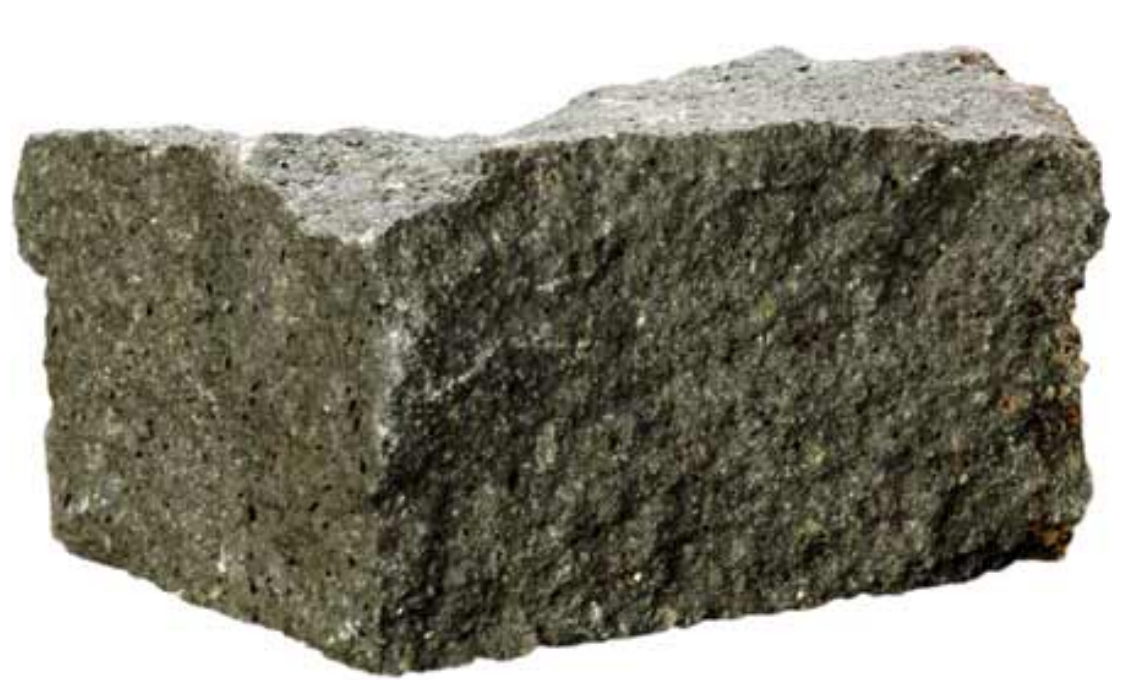
\includegraphics[width=0.6\textwidth]{figs/hw2fig0.png}
    \caption{\textbf{Example.} Starting with Step 1 of the classification table, we look at the structure of the rock. This one has crystals but no layers, so we go to step 3. At step 3, we look at the color of the crystals, which are mostly dark gray, so we go to step 5. At step 5, we check the color of the surrounding rock, which is also dark gray, so we go to step 6. Te rock is fine grained (no obvious crystal grains), so we conclude that the rock is \textbf{basalt}!}
    \label{fig:table1}
\end{figure}
\begin{figure}[h!]
    \centering
    \includegraphics[width=0.9\textwidth]{figs/hw2fig1.png}
    \label{fig:table1}
\end{figure}
\newpage
\noindent \textbf{Your assignment.}

Your task is to create a Python program that automates the process of navigating this table. You will develop an interface to ask the user questions about a given rock, use conditional statements to interpret those responses and navigate the above table, and finally output your identification of the type of rock.

\begin{enumerate}
    \item Start a new Colab notebook. Add a title and your name to the top of the notebook, and acknowledge resources used. Refer to class notebooks for examples about how to format your notebook so that it effectively communicates your work.
    \item Add a new text cell to outline your strategy for your code. Specifically discuss:
    \begin{itemize}
        \item How you plan to convert the \textit{go to} statements in the table into \textit{if} statements.
        \item Your strategy for prompting the user to provide input in a format that you can reliably process (capitalization? y/n vs yes/no vs Y/N, etc).
    \end{itemize}
    \item Add one or more code blocks to write your program to help a user identify a rock.
    \begin{itemize}
        \item Use the \verb!input! command to collect answers to your questions. Do not "hard code" answers - the program should respond case-by-case depending on the user input.
        \item At the end of the program, print out the type of rock (e.g. \verb~It's basalt!~).
        \item Feel free to break your code into multiple code blocks to help keep things organized and easier to debug. You can still run the entire program in order by clicking on \verb~Runtime < Run All~ if you don't want to click through individual blocks later. (Also remember \verb~Shift+Enter~ is a useful shortcut to evaluate blocks!)
    \end{itemize}
    \item Test your program on a few rocks.\\
    %\begin{centering}
    \includegraphics[width=0.9\textwidth]{figs/hw2fig2.png}\\
   % \end{centering}
    We will help you debug - when grading your code we will test on Diorite and Schist, but there will also be one mystery rock to make sure you can handle something arbitrary.
    \item For each of the above rocks, \textbf{insert the image into your notebook and copy the log and resulting identification from running your program. }
    \item Did you remember to acknowledge your collaborators?
    \item Submit your work as both an ipynb and pdf to Canvas.
\end{enumerate}

\end{document}